\documentclass{article}
\usepackage{tmlr}

% === Packages ===
\usepackage{amsmath, amssymb}
\usepackage{booktabs}
\usepackage{graphicx}
\usepackage{hyperref}
\usepackage{xcolor}
\usepackage{enumitem}
\usepackage{tikz}
\usetikzlibrary{arrows.meta, positioning}

\title{Benchmarks Are Engines, Not Cameras:\\Performativity, Proof Cultures, and the Social Production\\of Machine Learning Knowledge}

\author{
  Elliott Tower \and Donald MacKenzie\\
  University of Edinburgh\\
  \texttt{elliot@elliottower.ai}
}

\def\month{06}
\def\year{2026}

\begin{document}
\maketitle

\begin{abstract}
Machine learning benchmarks function as engines, not cameras: they reshape the practices they measure. Drawing on MacKenzie's sociology of financial models, we document three mechanisms by which benchmarks produce ML knowledge rather than merely recording it---performative adoption cycles, proof-culture fragmentation across subfields, and structural conditions for counterperformative peer review. Using citation analysis of 10 benchmark papers via OpenAlex, a manual comparison-count audit of 18 papers, and demand-compliance analysis of 11,196 ICLR submissions, we find that benchmark abandonment tracks social utility rather than scientific exhaustion; that mechanistic interpretability subfields accept incommensurable evidence standards for equivalent claims; and that reviewer experiment demands, added without comparison-count correction, structurally concentrate selective-reporting incentives in borderline submissions. Statistical reform treats the symptom. The cause is an evaluation culture whose instruments both measure and manufacture what counts as knowledge.
\end{abstract}


% ============================================================
%  1. INTRODUCTION
% ============================================================
\section{Introduction}

In 2006, MacKenzie argued that financial models are better understood as \textit{engines} that reshape markets than as \textit{cameras} that passively record them~\citep{mackenzie_engine_2006}. The Black-Scholes options-pricing model did not merely describe prices; traders adopted it, and prices came to conform to it --- a phenomenon MacKenzie termed \textit{Barnesian performativity}~\citep{mackenzie_millo_2003}. The model made itself true.

We argue that the same dynamic operates in machine learning research, with benchmarks playing the role of pricing models. ImageNet~\citep{deng_imagenet_2009} does not passively measure visual understanding; it defines what visual understanding \textit{means} for the research community, shapes training procedures, data collection, and career incentives, and is abandoned not when vision is ``solved'' but when a new benchmark captures the community's attention. GLUE~\citep{wang_glue_2018} did not measure natural language understanding; it measured the ability to fine-tune on a specific task distribution, and was replaced by SuperGLUE within two years. MMLU~\citep{hendrycks_mmlu_2021} arguably measures test-taking on multiple-choice questions more than it measures reasoning, and is already being supplemented by benchmarks that its creators argue more faithfully capture what MMLU was supposed to.

The benchmark is an engine, not a camera. And like the Gaussian copula whose widespread adoption created correlated fragility it could not represent~\citep{mackenzie_bamford_2018}, widespread optimisation against a benchmark can create overfitting it cannot detect.

The analogy is not that benchmarks and financial models are the same kind of object. They act through different channels. Option-pricing models reshaped markets through trading desks, arbitrage practices, risk systems, and regulatory acceptance. Benchmarks reshape machine learning through conference review criteria, leaderboards, dataset reuse, model-release announcements, lab hiring, grant narratives, and the everyday decision of what experiment to run next. A benchmark becomes performative when these channels make its score more than a measurement---the score becomes a reason to build one system rather than another.

Using a manual comparison-count audit of 12 landmark ML papers (Appendix~\ref{app:landmark_audit}), 6 mechanistic interpretability papers (Appendix~\ref{app:mi_audit}), citation-based trend analysis via OpenAlex~\citep{priem_openalex_2022}, and demand-compliance analysis of 11,196 ICLR submissions across 2023--2024, we document how this performative loop operates: benchmark adoption and abandonment patterns that track social utility rather than scientific exhaustion (Section~\ref{sec:performativity}); proof-culture fragmentation in mechanistic interpretability where subfields accept incommensurable evidence for mechanistic claims (Section~\ref{sec:proof_cultures}); and evidence from two years of ICLR submissions that the peer review system's demand-compliance dynamic creates structural conditions under which additional experiments are introduced without comparison-count adjustment (Section~\ref{sec:counterperformativity}). ML's evaluation failures are better understood as structural rather than individual---the publication system preferentially admits novel positive results and makes it harder to publish the replications, null findings, and modest corrections that would surface false positives.


% ============================================================
%  2. THEORETICAL FRAMEWORK
% ============================================================
\section{Theoretical Framework}
\label{sec:theory}

We draw on three strands of work from the sociology of science that have not previously been applied to ML evaluation methodology.

\subsection{Performativity}

MacKenzie~\citep{mackenzie_engine_2006} distinguishes three levels of performativity:

\begin{description}[leftmargin=1.5cm]
  \item[Generic] Practitioners use a theory or model in their work.
  \item[Effective] Use of the theory has a causal effect on the phenomenon it describes.
  \item[Barnesian] Use of the theory makes the world conform more closely to the model --- the strongest form, in which the map redraws the territory.
\end{description}

He also introduced, with Bamford, the concept of \textit{counterperformativity}: when a model's widespread adoption causes the world to diverge from the model's predictions, as when universal use of the Gaussian copula in credit risk created the very correlations the model assumed away~\citep{mackenzie_bamford_2018}.

\subsection{Cultures of Proving}

In his work on formal verification and mathematical proof, MacKenzie showed that what counts as a valid ``proof'' of a computer system's correctness is not a settled logical matter but a socially negotiated boundary between disciplinary communities --- logicians, mathematicians, and engineers accepted different kinds of arguments as constituting proof, with closure shaped by funding structures and regulatory demands rather than by epistemics alone~\citep{mackenzie_mechanizing_2001}.

\subsection{Performativity, Reflexivity, and Goodhart's Law}

Our use of performativity requires distinguishing it from two related concepts. \textit{Reflexivity} (Merton's self-fulfilling prophecy~\citep{merton_self_fulfilling_1948}) describes any case where a measurement affects what it measures. \textit{Goodhart's Law} (``when a measure becomes a target, it ceases to be a good measure'') describes optimization against a proxy metric. Both apply to ML benchmarks. Our claim is that performativity adds something specific: attention to the \textit{mechanism} by which models reshape social reality. In Callon's~\citep{callon_laws_1998} original formulation, performativity operates through the material and social infrastructure that translates a model into practice. MacKenzie's contribution was to show that this process has degrees (generic, effective, Barnesian) and can fail (counterperformativity).

For ML benchmarks, we claim \textit{effective} performativity, not Barnesian: benchmarks causally reshape research priorities, training procedures, and career incentives, but we do not claim that the world comes to conform to the benchmark's implicit model in the strong sense that options prices came to conform to Black-Scholes. The closest analogy is Espeland and Sauder's~\citep{espeland_sauder_2007} analysis of law school rankings, where the rankings reshaped law school behaviour---admissions criteria, resource allocation, strategic gaming---without making law schools conform to an underlying formal model.

We anticipate the objection that performativity is ``just Goodhart's Law with fancier vocabulary.'' The distinction is substantive: Goodhart tells you \textit{that} a metric will degrade; performativity identifies the \textit{mechanism}---which institutional channels sustain the degradation, and why it is self-reinforcing. The critical addition is counterperformativity: the prediction that a safety mechanism can generate the risk it is designed to prevent, a dynamic Goodhart cannot describe. Section~\ref{sec:counterperformativity} provides empirical evidence for this in the peer review system.

\subsection{Publication Bias and Structural Selection}

The replication crisis literature has documented three stacked asymmetries in the publication system~\citep{franco_publication_2014, simonsohn_p_curve_2014}:

\begin{enumerate}[leftmargin=*]
  \item \textbf{Positive-results bias.} Journals overwhelmingly accept positive, novel findings; null results are not published.
  \item \textbf{Anti-replication bias.} Reviewers treat replication studies as ``not novel'' regardless of their scientific value.
  \item \textbf{Gotcha bias.} Disproofs are publishable only when they dramatically overturn a famous result --- modest corrections are rejected as ``not surprising.''
\end{enumerate}

Together, these create a one-sided filter: the very outputs that would correct the literature's false-positive accumulation are the outputs the system tends to reject.


% ============================================================
%  3. DATA AND METHODS
% ============================================================
\section{Data and Methods}
\label{sec:methods}

\subsection{OpenReview Demand-Compliance Analysis}

To provide direct evidence for the counterperformativity of peer review (Section~\ref{sec:counterperformativity}), we analysed all publicly available submissions to ICLR 2024 ($n = 7{,}404$) and ICLR 2023 ($n = 3{,}792$), retrieved via the OpenReview REST API. For each venue, we extracted (i)~explicit experiment demands from reviewer text using keyword patterns for ablation requests, seed/variance demands, baseline additions, and dataset expansions; (ii)~author compliance signals from rebuttals (e.g., ``we added new experiments,'' ``we have updated the manuscript''); and (iii)~final acceptance decisions. This pipeline allows us to trace the association between reviewer demands, author compliance, and publication outcomes across two years of the same venue. We note that this is an observational study: papers that comply may differ systematically from those that do not (e.g., in lab resources or initial quality). We report the association as evidence for a structural pattern.

\subsection{OpenAlex Citation Analysis}

We use structured citation metadata from OpenAlex~\citep{priem_openalex_2022} to track two trends via citation links (not keyword matching): (i)~benchmark lifecycle curves, measuring year-by-year citation counts for 10 major benchmark-introducing papers to quantify adoption and abandonment patterns; and (ii)~statistical correction adoption rates, measuring the fraction of ML papers per year that cite the canonical papers introducing Bonferroni~\citep{dunn_1961}, Holm~\citep{holm_1979}, or Benjamini-Hochberg~\citep{benjamini_hochberg_1995} corrections. The ML paper population is defined as works tagged with the ``Machine learning'' concept in OpenAlex.

\subsection{Case Studies}

We develop three detailed case studies:
\begin{enumerate}[leftmargin=*]
  \item \textbf{ImageNet} (2009--present): the canonical performativity cycle, from benchmark to engine to cultural institution.
  \item \textbf{GLUE $\to$ SuperGLUE $\to$ MMLU}: the accelerating benchmark replacement cycle in NLP.
  \item \textbf{Mechanistic interpretability proof cultures}: the fragmentation of validity standards across SAE, causal abstraction, and circuit-discovery communities (2022--2025).
\end{enumerate}

\subsection{Transparency Note}

We document our own file drawer in Section~\ref{sec:discussion}: analyses attempted during development that do not appear in the final paper, including failed venue replications and abandoned methodologies.


% ============================================================
%  4. BENCHMARK PERFORMATIVITY
% ============================================================
\section{Benchmarks as Engines}
\label{sec:performativity}

\subsection{The Performativity Cycle}

We observe a recurring four-phase cycle in benchmark adoption:

\begin{enumerate}[leftmargin=*]
  \item \textbf{Introduction (camera phase).} A benchmark is proposed as a measurement instrument for a capability (visual recognition, language understanding, reasoning). At introduction, it functions as a camera: it passively records model performance.
  \item \textbf{Adoption (generic performativity).} Researchers begin optimising against the benchmark. Papers report scores. Leaderboards emerge. The benchmark's scores become the operational definition of the capability it was designed to measure.
  \item \textbf{Saturation (effective performativity).} Optimisation against the benchmark changes training procedures, data collection, and architecture choices. The benchmark's use has a causal effect on the phenomenon: models get better \textit{at the benchmark}, which may or may not correspond to improvement in the underlying capability. Transfer studies (e.g., \citealt{recht_imagenet_2019}) begin revealing the gap.
  \item \textbf{Abandonment or replacement (counterperformativity).} The benchmark is either saturated (human-level accuracy is reached, rendering further comparison meaningless) or recognised as no longer measuring what it was supposed to (the engine has diverged too far from the territory). A new benchmark is introduced, and the cycle restarts.
\end{enumerate}

Citation-based lifecycle data from OpenAlex (Table~\ref{tab:lifespans} and Figure~\ref{fig:lifecycle}a) confirms that NLP benchmarks complete this cycle faster than vision benchmarks. GLUE peaked in 2023 at 1,052 citations per year and dropped 54\% by 2024; SuperGLUE peaked the same year and dropped 69\%. ImageNet peaked in 2021 at 9,305 citations per year but declined only 16\% by 2024, sustained by its role as a pretraining dataset and cultural reference point even as new benchmarks emerge. A caveat: citation counts conflate usage, critique, and passing mention. A paper that critiques ImageNet cites it; a paper so familiar with ImageNet that it uses the dataset without comment may not. The decline trends are therefore a noisy proxy for adoption, not a direct measure of it. We report them as evidence of shifting community attention, not as proof of abandonment.

\begin{table}[t]
\centering
\caption{Benchmark performativity cycles, measured by year-over-year citation counts from OpenAlex. Decline is measured from peak year to 2024. NLP benchmarks complete the camera$\to$engine transition in 3--5 years; vision benchmarks persist for 10+.}
\label{tab:lifespans}
\small
\begin{tabular}{@{}lccrrc@{}}
\toprule
Benchmark & Domain & Intro & Peak year & Peak cites/yr & Decline to 2024 \\
\midrule
GLUE & NLP & 2018 & 2023 & 1{,}052 & $-$54\% \\
SuperGLUE & NLP & 2019 & 2023 & 359 & $-$69\% \\
SQuAD & NLP & 2016 & 2021 & 1{,}237 & $-$59\% \\
\midrule
ImageNet & Vision & 2009 & 2021 & 9{,}305 & $-$16\% \\
CIFAR-10 & Vision & 2009 & 2021 & 4{,}870 & $-$39\% \\
\midrule
MMLU & LLM & 2021 & 2023 & 133 & $-$24\% \\
HumanEval & Code & 2021 & 2023 & 604 & $-$35\% \\
HELM & LLM & 2022 & 2023 & 146 & $-$15\% \\
\bottomrule
\end{tabular}
\end{table}

\begin{figure}[t]
\centering

\includegraphics[width=\textwidth]{fig_lifecycle.pdf}
\caption{(a)~Benchmark adoption and abandonment measured by citations per year from OpenAlex. NLP benchmarks (GLUE, SuperGLUE, SQuAD) spike and crash within 3--5 years; vision benchmarks (ImageNet, CIFAR-10) persist for 10+ years as cultural institutions. (b)~Statistical correction adoption in ML, measured as the fraction of ML papers per year citing the canonical papers introducing Bonferroni, Holm, and Benjamini-Hochberg corrections. Adoption is not merely low but \emph{declining}, from 0.17\% to 0.09\% for Benjamini-Hochberg between 2015 and 2025.}
\label{fig:lifecycle}
\end{figure}

\subsection{Counterperformativity: When Benchmarks Break}

The counterperformative moment --- when widespread adoption of a model causes it to fail --- has a specific signature in ML: the benchmark is revealed to be testing something other than what it is named after. MMLU tests multiple-choice test-taking, not ``massive multitask language understanding.'' GLUE tested fine-tuning ability, not ``general language understanding.'' The name persists after the measurement has diverged from it, creating a gap between the benchmark's name and what its scores appear to reflect.

This is the Gaussian copula dynamic transplanted into research evaluation. Widespread optimisation against a benchmark can create overfitting the benchmark itself cannot detect, because the benchmark \textit{is} the detection instrument.


% ============================================================
%  6. PROOF CULTURES IN ML
% ============================================================
\section{Proof Cultures and Their Fragmentation}
\label{sec:proof_cultures}

\subsection{Three Proof Cultures in Mechanistic Interpretability}

The emerging subfield of mechanistic interpretability --- the attempt to reverse-engineer the internal computations of neural networks --- provides a particularly clear case of proof-culture fragmentation. We identify at least three communities operating with distinct and largely incommensurable standards for what constitutes a valid mechanistic claim:

\begin{description}[leftmargin=*]
  \item[Sparse autoencoders (SAE).] Validity is established by demonstrating that learned features are monosemantic (respond to one interpretable concept), sparse, and reconstructive of model activations. The proof standard is \textit{feature-level}: a mechanism is valid if its component features are interpretable.
  \item[Causal abstraction.] Validity is established by showing that an interpretive model is causally aligned with the neural network under interchange interventions~\citep{geiger_causal_2021}. The proof standard is \textit{intervention-level}: a mechanism is valid if intervening on the proposed variables produces the predicted effect on behaviour.
  \item[Circuit discovery.] Validity is established by identifying subgraphs of the network that are sufficient to reproduce behaviour on a task, typically via activation patching or edge attribution. The proof standard is \textit{sufficiency-level}: a mechanism is valid if the identified circuit is sufficient and necessary for the behaviour.
\end{description}

The difference becomes visible in what each community treats as a persuasive figure. In an SAE paper, the persuasive object is typically a feature dashboard: activating examples, a natural-language label, and a sparse set of tokens that make the feature feel semantically coherent. In a causal-abstraction paper, the persuasive object is an intervention result: replacing a proposed variable changes model behaviour in the way the abstraction predicts. In a circuit-discovery paper, the persuasive object is a subgraph: a set of heads or edges whose removal changes task performance. These are not interchangeable evidential forms. Each makes a different kind of object visible and leaves a different kind of uncertainty in the background.

They also reflect different ontological commitments about what a ``mechanism'' is. The SAE community treats mechanisms as collections of features. The causal abstraction community treats them as causal models. The circuit community treats them as computational subgraphs. These are, in MacKenzie's terminology, different \textit{cultures of proving} --- and the boundary between them appears to be shaped as much by institutional authority and funding patterns as by experimental evidence.

A citation analysis of 27 canonical MI papers across the three communities confirms this fragmentation empirically: SAE and causal-abstraction papers share only 1 cross-citation across 72 possible directed paper pairs (1.4\% density), despite both communities citing the foundational circuit-discovery literature heavily (19 combined edges). The pattern is two newer proof cultures building independently on the same older foundation without citing each other.\footnote{The citation analysis covers $\sim$9 SAE, $\sim$8 causal abstraction, and $\sim$10 circuit discovery papers (2020--2025), retrieved via Semantic Scholar and OpenAlex APIs. The sample captures canonical papers; the full MI literature may show denser cross-citation at the periphery. Temporal asymmetry (circuits papers predate SAE/causal work) explains the absence of reverse citations from circuits to newer communities.}

\subsection{The Social Production of Fragmentation}

Why don't these communities converge? The interdisciplinarity literature suggests an answer: convergence is structurally disincentivised. Junior researchers face career risk from interdisciplinary work~\citep{leahey_prominent_2017}. Grant proposals include other perspectives ``only superficially, mostly to increase the chance of being funded''~\citep{klein_interdisciplinarity_2010}. The reward structure makes monodisciplinary specialisation the dominant strategy even when the problem demands range~\citep{epstein_range_2019}.

The result is that proof-culture fragmentation in mechanistic interpretability is not a temporary state awaiting the right unifying experiment. The incentive structure suggests it may be self-sustaining, maintained by the same publication and career incentives that drive the evaluation culture's other pathologies. MacKenzie's Strong Programme analysis applies: the \textit{content} of mechanistic interpretability knowledge (fragmented, with plural proof standards) is causally shaped by the \textit{social conditions} of its production.

\subsection{The Denominator Problem in Practice}

The fragmentation described above has a concrete empirical consequence. The SAE proof culture, in particular, introduces a distinctive and largely unrecognised multiple comparison problem. A sparse autoencoder trains a dictionary of $N$ features (typically $N = 4{,}096$ to $34{,}000{,}000$), each of which is implicitly tested for interpretability. The researcher examines features, selects the $k \ll N$ that appear most interesting, and reports those as evidence that the method ``finds interpretable features.'' This is a multiple hypothesis test with $m \geq N$, and none of the six MI papers we audited corrects for it.

A manual FWER audit of six MI papers (Appendix~\ref{app:mi_audit}) finds implied comparisons ranging from 12,000 (Bricken et al.\ 2023, dictionary of 4,096) to 170,000,000 (Templeton et al.\ 2024, dictionary of 34M). The Bonferroni threshold for the largest case is $\alpha^* = 2.9 \times 10^{-10}$---no interpretability metric in the literature comes close.

The fix is to report the interpretability \textit{rate}: the fraction of features passing a threshold, not just the highlighted examples. Recent tools make this tractable. SAEBench~\citep{karvonen_saebench_2025} scores each latent by asking an LLM to identify activating sequences from a feature description, yielding scores between 0 and 1. On a Pythia-70M SAE (100 randomly sampled latents), the mean score is 0.84 (SD = 0.12), and 92\% of features score above 0.7. At production scale, a different failure mode appears: Paulo et al.~\citep{paulo_autointerp_2024} scored millions of features on a 131K-feature Gemma-2 9B SAE and found that 30\% of features do not activate frequently enough to generate the examples the scoring method requires. This is not the same as low interpretability---it is a coverage problem, where the evaluation instrument cannot reach a substantial fraction of the dictionary. The two failure modes compound: features that do activate may score well; features that rarely activate are unmeasurable; and the published interpretability rate reflects only the former. Publishing full score distributions, pass rates at standard thresholds, and activation-coverage fractions should be a required reporting metric.

The feature-selection problem is not only statistical. It is also evidential. SAE papers persuade through curated visibility: the reader is shown features that appear coherent, memorable, and nameable. The denominator remains offstage. This is not a failure of individual honesty; it is part of the proof culture. The dashboard, the highlighted feature, and the vivid label function as demonstrations---they make a mechanism available to perception. But precisely because they work visually, they can make selection disappear. The risk is not hypothetical: Adebayo et al.~\citep{adebayo_sanity_2018} demonstrated that several prominent saliency methods produce identical outputs regardless of whether the model has been trained---the visual persuasiveness of the explanation was independent of whether the model had learned anything. As Marks~\citep{marks_illusory_2025} observes informally, ``there's inherently a bit of a lag between new types of claims being made, and having an experimental paradigm suited to validating them.'' The ablation controls that now catch such illusions in saliency maps do not yet exist for SAE feature dashboards.

Moreover, the denominator is itself unstable. Paulo and Belrose~\citep{paulo_belrose_seeds_2026} showed that SAEs trained on the same model and data with different random seeds learn fundamentally different features: in a 131K-latent SAE on Llama~3 8B, only 30\% of features were shared across seeds. As they conclude, ``the set of features uncovered by an SAE should be viewed as a pragmatically useful decomposition of activation space, rather than an exhaustive and universal list of features `truly used' by the model.'' The reported features are a selected subset of an unstable decomposition---the denominator is not merely large but indeterminate. Whether the monosemantic feature is discovered by the decomposition or produced by it remains an open question.

\paragraph{A worked example: Templeton et al.\ (2024).} The selection problem is most vivid in the largest published SAE study. Templeton et al.\ trained a dictionary of 34,000,000 features on Claude 3 Sonnet and presented approximately 10 features in detail---a selection ratio of 3.4 million to one. The presented features are striking: one activates on mentions of the Golden Gate Bridge, another on code syntax errors, another on sycophantic praise. Each is accompanied by activation examples, steering demonstrations, and qualitative interpretation. The evidential force of this presentation depends entirely on the denominator. If 10 features were selected from 34 million, the question is not whether those 10 are interpretable---it is how many of the remaining 33,999,990 would \textit{also} appear interpretable if examined with equal care. If even 0.01\% of features are spuriously interpretable (e.g., because they correlate with common input patterns), that yields 3,400 false positives---dwarfing the 10 that are shown. The paper does not report how many features were examined before the presented subset was selected, because the proof culture does not require it. If Bonferroni correction were applied to the full dictionary, the significance threshold would be $\alpha^* = 1.5 \times 10^{-9}$; no interpretability metric in the literature comes close. We do not argue that these features are spurious. We argue that the evidence cannot distinguish real features from spurious ones at the reported selection ratio, and that reporting the denominator would make this distinction possible.

\paragraph{A positive control: Paulo and Belrose (2026).} The same Paulo and Belrose seed-stability study is the closest analogue to proper denominator reporting in the MI literature. Rather than selecting a favorable decomposition and curating its most compelling features, they compared decompositions across random seeds and reported the selection instability directly: only 30\% of features survived. This result reduces the epistemic weight of any single SAE training run---which is exactly what denominator reporting is supposed to do. It is the correct template: disclose the instability, let the reader assess the evidential weight, and accept that the finding may be less dramatic than a curated dashboard suggests.

\paragraph{A cross-field precedent.} The denominator problem is not unique to SAEs. Bolukbasi et al.\ \citep{bolukbasi_man_2016} evaluated word-embedding debiasing on the analogy task used to define the gender direction---the metric was constructed from the same distribution the debiasing was applied to. The method accumulated 2,685+ citations and was adopted as a preprocessing step in downstream NLP systems before Gonen and Goldberg \citep{gonen_lipstick_2019} showed, via clustering and classifier recovery, that the bias was geometrically intact: the debiasing had removed the projection most visible to the original evaluation while leaving relational structure untouched. The failure mode is precisely denominator selection: evaluating on the cases the method was optimised to handle, and treating success there as evidence for the full claim.

\subsection{The File Drawer Made Visible}

The de facto research methodology in MI --- described explicitly by one of the field's leading practitioners as a sequence of ``Explore $\to$ Understand $\to$ Distill''~\citep{nanda_research_process_2023} --- structurally guarantees the file-drawer problem. The exploration stage, which represents the majority of experimental activity, is explicitly designed not to appear in the written output. The distillation stage involves retroactively compressing exploration into a legible narrative. The experiments that didn't work disappear by design, not by accident.

A rare exception illustrates the mechanism by contrast. In 2025, the Google DeepMind MI team published a blog post explicitly framed as ``research we didn't consider a good fit for turning into a paper''~\citep{smith_gdm_negative_2025}, reporting negative results from SAE research: failed out-of-distribution probing, composition issues, absorption, missing features, and low sensitivity. Under the standard publication filter, all of this would have remained invisible. The decision to publish required a deliberate, non-standard intervention. The default --- for every team that ran similar experiments and wrote nothing --- was silence. The population of invisible file drawers is, by definition, unknown.


% ============================================================
%  7. THE COUNTERPERFORMATIVITY OF PEER REVIEW
% ============================================================
\section{The Counterperformativity of Peer Review}
\label{sec:counterperformativity}

The publication system introduces a final counterperformative dynamic that closes the loop. Reviewers, acting in good faith, demand additional experiments to increase confidence in a result: ``run three more seeds,'' ``add two baselines,'' ``test on another dataset.'' Each demand is intended to \textit{reduce} the false-positive rate. But each demanded experiment is a new fork in the garden of forking paths --- a fresh implicit comparison whose result will be selectively reported (the paper is revised to incorporate only the experiments that support the claim).

The \textit{mechanism} by which this could inflate false positives is straightforward: each demanded experiment is a new comparison whose result will be selectively reported (the paper is revised to incorporate supporting results). Whether this mechanism operates at scale is an empirical question we cannot definitively answer with observational data. But the structural conditions for it are present: the demand-compliance exchange is public, routine, and unaccompanied by any adjustment for the additional comparisons introduced.

This parallels the structure of MacKenzie and Bamford's counterperformativity: the model (more experiments = more confidence) is widely adopted, and its adoption creates conditions under which the phenomenon (false-positive rate) could diverge from the model's prediction (that more experiments should decrease it). We do not claim this divergence has been demonstrated---only that the structural conditions are visible in the review record and that the analogy to financial counterperformativity is precise enough to warrant attention.

\subsection{Empirical Evidence: The Demand-Compliance Pipeline}

The point is not that reviewers are cynical or that authors are deceptive. The demand-compliance exchange is public, routine, and usually conducted in good faith. A reviewer identifies an evidential gap; an author produces an additional experiment; the exchange becomes legible as rigour. Peer review does not merely evaluate the evidential record. It helps produce the record that it then evaluates. We trace this dynamic empirically using the complete public review corpora of ICLR 2024 ($n = 7{,}404$) and ICLR 2023 ($n = 3{,}792$).

Table~\ref{tab:demand_compliance} presents the aggregate results for both years. Table~\ref{tab:stratified} presents the same data stratified by mean reviewer score.

\begin{table}[t]
\centering
\caption{Demand--compliance--outcome pipeline at ICLR (aggregate). The compliance lift replicates across years: $+$10.7\,pp in 2024 and $+$13.0\,pp in 2023.}
\label{tab:demand_compliance}
\small
\begin{tabular}{@{}lrrrr@{}}
\toprule
 & \multicolumn{2}{c}{ICLR 2024 ($n = 7{,}404$)} & \multicolumn{2}{c}{ICLR 2023 ($n = 3{,}792$)} \\
\cmidrule(lr){2-3} \cmidrule(lr){4-5}
Condition & Papers & Accept\% & Papers & Accept\% \\
\midrule
No demands received & 5{,}063 & 39.7\% & 3{,}435 & 41.9\% \\
Demands received & 717 & 34.9\% & 357 & 37.3\% \\
\quad Complied & 177 & 42.9\% & 78 & 47.4\% \\
\quad Did not comply & 540 & 32.2\% & 279 & 34.4\% \\
\midrule
Compliance lift & \multicolumn{2}{c}{$+$10.7\,pp} & \multicolumn{2}{c}{$+$13.0\,pp} \\
\bottomrule
\end{tabular}
\end{table}

\begin{table}[t]
\centering
\caption{Score-stratified demand--compliance analysis (ICLR 2024, $n = 5{,}780$ matched with reviewer scores). The aggregate $+$10.7\,pp compliance lift is a Simpson's paradox: within score strata, the lift is small (borderline), absent (low, high), or \emph{negative} (mid). Compliant papers are disproportionately borderline; non-compliant papers are disproportionately low-scored.}
\label{tab:stratified}
\small
\begin{tabular}{@{}lccc@{}}
\toprule
Score stratum & Comply accept\% & No-comply accept\% & Lift \\
\midrule
Low ($< 4.5$) & 0.0\% ($n = 15$) & 0.0\% ($n = 155$) & 0.0\,pp \\
Borderline (4.5--5.5) & 7.5\% ($n = 53$) & 4.7\% ($n = 150$) & $+$2.9\,pp \\
Mid (5.5--6.5) & 50.0\% ($n = 70$) & 54.7\% ($n = 139$) & $-$4.7\,pp \\
High ($\geq 6.5$) & 94.9\% ($n = 39$) & 94.8\% ($n = 96$) & $+$0.1\,pp \\
\midrule
Aggregate & 42.9\% ($n = 177$) & 32.2\% ($n = 540$) & $+$10.7\,pp \\
\bottomrule
\end{tabular}
\end{table}

\paragraph{The aggregate lift is a composition effect.} The headline $+$10.7\,pp compliance lift in Table~\ref{tab:demand_compliance} is a Simpson's paradox. Table~\ref{tab:stratified} stratifies the same data by mean reviewer score and reveals that within score strata, the lift is small, absent, or reversed: low-scored papers are rejected regardless of compliance (0\% for both); mid-scored papers show compliant authors accepted at \emph{lower} rates ($-$4.7\,pp); high-scored papers are accepted at $\sim$95\% regardless. Only in the borderline stratum (mean score 4.5--5.5) does compliance show a positive association ($+$2.9\,pp), and even there the sample is small ($n = 53$ compliant). The ICLR 2023 data show a similar pattern: compliance lift concentrates in the borderline stratum ($+$13.3\,pp, but $n = 16$) and vanishes elsewhere.

The aggregate lift arises because compliant papers are disproportionately borderline (they received demands because reviewers were on the fence and compliance tipped them across), while non-compliant papers are more concentrated in the low stratum where nothing helps.

\paragraph{This sharpens the counterperformativity argument.} The incentive to comply selectively---running the demanded experiment and reporting only the supporting result---is strongest precisely for borderline papers, where a small shift in perceived rigour can change the decision. The review system concentrates the compliance reward at the margin where selective reporting is most tempting and least detectable. For low-scored papers, compliance is futile; for high-scored papers, unnecessary. The borderline stratum is where the counterperformative mechanism has the most bite.

\paragraph{Demand targets are weaker papers.} Papers that receive explicit experiment demands are accepted at lower rates than papers without demands (34.9\% vs.\ 39.7\% in 2024; 37.3\% vs.\ 41.9\% in 2023). The papers that attract demands are, on average, the papers the review system is already sceptical about. This is consistent with the pedagogical function of demanding experiments: reviewers use experiment demands as a structured way to express scepticism.

\paragraph{The reward is for effort, not evidence.} The most common demands --- ablation studies, seeds and variance reporting, and additional baselines --- are precisely the kinds of experiments that increase the number of implicit comparisons without altering the paper's central claim. An author who runs an additional ablation and reports the result has added a fork in the garden of forking paths. The review system rewards this fork as \textit{evidence of rigour}. But the fork was introduced \textit{after} the result was known, and only the supporting outcome is reported in the revised manuscript.

\paragraph{Typical demand and compliance language.} The texture of the demand-compliance interaction reveals its performative character. Reviewers write: ``The ablation studies are lacking. It is hard to see where the performance gains come from''; ``Standard deviations are not reported in Table 2, Table 3, Table 4''; ``it would be beneficial to include a comparison with more state-of-the-art IL methods.'' Authors respond: ``we added new experiments, showing that our approach outperforms all baselines''; ``we have modified the paper to include clean accuracy on the CIFAR-10 dataset as well.'' The rhetorical structure is consistent: the demand is framed as a gap in rigour, and the compliance is framed as having filled that gap.

\subsection{The Counterperformative Loop, Quantified}

These findings are consistent with the counterperformative loop diagrammed in Figure~\ref{fig:loop}, though they do not prove it. The review system's operating model is that demanding more experiments should increase confidence and decrease the false-positive rate. Score-stratified analysis (Table~\ref{tab:stratified}) reveals that the aggregate compliance lift is a composition effect---a Simpson's paradox driven by the concentration of compliant papers in the borderline score stratum. Within strata, compliance provides little or no advantage.

We emphasise what the data can and cannot show. The stratified results are consistent with two interpretations: compliance has no causal effect and the aggregate lift is a pure compositional artifact, or compliance has a small real effect concentrated in borderline submissions. Our argument does not depend on which is true---both are consistent with the structural conditions we identify, and both are predicted by the counterperformativity framing. The association between compliance and acceptance in the borderline stratum ($+$2.9\,pp, $n = 53$) is small and compatible with a mundane explanation: compliant borderline papers may simply be better papers with more resources. The data cannot distinguish selective reporting from genuine evidential improvement. What the data \textit{do} show is a structural pattern: the compliance incentive concentrates where selective reporting would be most consequential, and the demanded experiments are introduced without any framework for adjusting the comparison count. The replication across two years of the same venue suggests the pattern is stable, not an artefact of a single cohort.


\begin{figure}[t]
\centering
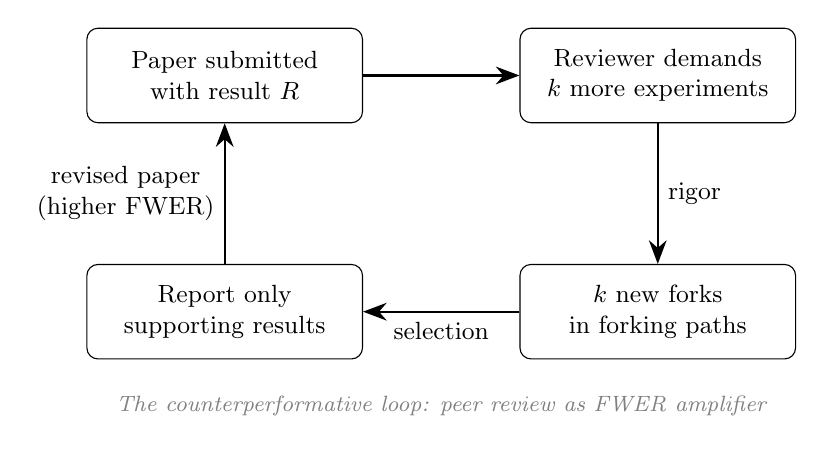
\begin{tikzpicture}[
  box/.style={draw, rounded corners, minimum width=3.5cm, minimum height=1.2cm, align=center, font=\small},
  arr/.style={-{Stealth[length=3mm]}, thick},
  every node/.style={font=\small}
]
  \node[box] (submit) at (0,0) {Paper submitted\\with result $R$};
  \node[box] (review) at (5.5,0) {Reviewer demands\\$k$ more experiments};
  \node[box] (fork) at (5.5,-3) {$k$ new forks\\in forking paths};
  \node[box] (select) at (0,-3) {Report only\\supporting results};

  \draw[arr] (submit) -- (review);
  \draw[arr] (review) -- node[right] {rigor} (fork);
  \draw[arr] (fork) -- node[below] {selection} (select);
  \draw[arr] (select) -- node[left, align=center] {revised paper\\(higher FWER)} (submit);

  \node[font=\footnotesize\itshape, text=gray] at (2.75, -4.2) {The counterperformative loop: peer review as FWER amplifier};
\end{tikzpicture}
\caption{The structural conditions for counterperformativity in peer review. Each cycle of reviewer-demanded experiments increases the number of implicit comparisons without adjusting the comparison count. Our ICLR analysis of 11,196 submissions across 2023--2024 shows that the aggregate compliance--acceptance association is a Simpson's paradox: it concentrates in the borderline score stratum, where the incentive for selective reporting is strongest. The data show the structural pattern; whether it inflates false positives in practice is not directly observable.}
\label{fig:loop}
\end{figure}


% ============================================================
%  BENCHMARK PERFORMATIVITY BEYOND RESEARCH
% ============================================================
% ============================================================
%  RELATED WORK
% ============================================================
\section{Related Work}
\label{sec:related}

The performativity of evaluation instruments has been explored in several adjacent literatures. In education, the literature on ``teaching to the test'' documents how standardised assessments reshape curricula to optimise for the instrument rather than the underlying capability~\citep{au_high_2007}. In economics, Goodhart's Law --- ``when a measure becomes a target, it ceases to be a good measure'' --- is the most-cited reference for this argument in computer science~\citep{goodhart_1975}. Goodhart describes the symptom: measures captured by their use. Performativity theory describes the mechanism: how the use of a measure recursively reshapes what the measure can detect, and how counterperformativity creates the specific failure mode in which the safety apparatus generates the risk it was designed to prevent.

Most directly relevant to our analysis is Koch and Peterson's~\citep{koch_peterson_2024} study of how benchmarking practices in ML have contributed to ``epistemic monoculture'' --- the narrowing of research diversity as the community converges on a small set of evaluation instruments, datasets, and methods. Their work combines qualitative interviews with ML researchers and computational analysis of publication patterns to show that benchmarking creates self-reinforcing cycles of methodological convergence. Our analysis extends Koch and Peterson's in two directions: first, we ground the monoculture dynamic in MacKenzie's performativity framework, providing a theoretical vocabulary (generic, effective, Barnesian, and counterperformative) for the mechanisms they describe; second, we provide quantitative evidence from the review process itself --- the demand-compliance pipeline of Section~\ref{sec:counterperformativity} --- showing that the peer review system actively rewards compliance with the monoculture's proof standards rather than passively reflecting them.

Within ML, several recent papers have identified specific evaluation failures. Dehghani et al.~\citep{dehghani_benchmark_2021} document the ``benchmark lottery''---how arbitrary choices in benchmark construction determine which methods appear superior---but do not theorize why the lottery persists institutionally. Bowman and Dahl~\citep{bowman_what_2021} catalogue what it would take to fix NLP benchmarking (dynamic benchmarks, comprehensive evaluation, richer metrics) but do not explain why the field has not adopted these fixes despite knowing about them for years. Raji et al.~\citep{raji_ai_2021} argue that the AI benchmark ecosystem lacks the accountability infrastructure of standardized testing in other domains. Our analysis extends these critiques by providing a theoretical framework---performativity---that explains \textit{why} the known problems persist: benchmark degradation is not a bug to be fixed but a structural feature of how evaluation instruments interact with the incentive systems that surround them.

The replication crisis literature in psychology~\citep{nosek_replication_2015} and biomedicine~\citep{ioannidis_2005} has extensively documented the consequences of publication bias, $p$-hacking, and selective reporting, but has primarily focused on statistical remedies (preregistration, effect size reporting, $p$-curve analysis). Our contribution is to show that ML's evaluation failures have a specifically \textit{structural} character that statistical remedies alone cannot address: the publication system selects against the very outputs (replications, null results, modest corrections) that would surface the false positives statistical methods are designed to catch.


% ============================================================
%  9. DISCUSSION
% ============================================================
\section{Discussion: Why Statistical Reforms Alone Are Insufficient}
\label{sec:discussion}

Statistical interventions --- Bonferroni corrections, preregistration, confidence intervals, seed averaging --- treat the problem as a deficit of rigour on the part of individual researchers. Our data suggest a different diagnosis. The problem is not that researchers have failed to apply statistics correctly. It is that the publication system selects against the very outputs that statistics is designed to produce: replications, null results, and modest corrections.

Citation-based evidence from OpenAlex reinforces this structural diagnosis (Figure~\ref{fig:lifecycle}b). Tracking ML papers that cite the canonical papers introducing Bonferroni~\citep{dunn_1961}, Holm~\citep{holm_1979}, and Benjamini-Hochberg~\citep{benjamini_hochberg_1995} corrections, we find that correction adoption is not merely low but \emph{declining} as a fraction of total ML output: Benjamini-Hochberg citations dropped from 0.17\% of ML papers in 2019 to 0.09\% in 2025; Holm from 0.06\% to 0.01\%; Bonferroni from 0.03\% to 0.01\%. The statistical corrections exist. The field is not adopting them, and the trend is negative. This is not a knowledge gap---it is a structural selection pressure that makes correction invisible to the reward system.

\subsection{How Large Is the Inflation?}

Our comparison-count audits (Appendices~\ref{app:landmark_audit} and~\ref{app:mi_audit}) give concrete denominators. The median landmark paper contains 414 implicit comparisons. What does that actually buy you?

From order statistics: if you pick the best of $N$ independent draws from noise with standard deviation $\sigma$, the winner's expected inflation is $\sigma\sqrt{2 \ln N}$. At $N = 414$, that is roughly $3.5\sigma$. But the i.i.d.\ assumption overstates the case: hyperparameter configurations within a paper are correlated (same dataset, overlapping architectures, shared training infrastructure), so the effective number of independent comparisons $N_{\text{eff}}$ may be much smaller. For sensitivity: at $N_{\text{eff}} = 40$ (a tenfold reduction), expected inflation drops to $\sigma\sqrt{2 \ln 40} \approx 2.7\sigma$; at $N_{\text{eff}} = 10$, to $\sigma\sqrt{2 \ln 10} \approx 2.1\sigma$. The direction is unambiguous across the plausible range, and the magnitude is unknowable without the denominator---which is exactly why reporting comparison counts matters.

From information theory: reporting $k$ results from $N$ candidates discards $\log_2\binom{N}{k}$ bits about the search. For the median landmark paper ($N = 414$, reporting $\sim$15 key results), that is roughly 80 bits---the entropy of 80 coin flips. The reader sees the outcomes; the process that selected them is gone.

\subsection{Other Fields Responded to This}

We surveyed seven fields that have faced the same problem. Table~\ref{tab:cross_field} summarises how each responded. A caveat: none of these reforms is uncontested or complete.

\begin{table}[t]
\centering
\caption{Multiple comparison problems across empirical fields. SAE feature selection operates at the highest dimensionality and is the only case with no correction norm.}
\label{tab:cross_field}
\small
\begin{tabular}{@{}llll@{}}
\toprule
\textbf{Field} & \textbf{Search space} & \textbf{FDR / Replication} & \textbf{Response} \\
\midrule
fMRI voxels & 130K & $>$80\% regional FDR & FWER/FDR mandatory \\
Candidate genes & $\sim$1000s & 1.2\% replication & GWAS replaced candidates \\
Finance factors & 316+ & 58\% post-pub decline & $t > 3.0$ proposed \\
Psychology & 34 DFs & 36\% replication & Preregistration \\
Drug discovery & 1000s & 92.6\% preclinical FDR & Target validation \\
Radiomics & 100s--1000s & Pipeline-dependent & Harmonization (IBSI) \\
SAE features & 16K--131K & 30\% seed stability & \textbf{None yet} \\
\bottomrule
\end{tabular}
\end{table}

The fMRI case is the most structurally parallel. Bennett et al.~\citep{bennett_dead_salmon_2010} scanned a dead Atlantic salmon and found statistically significant ``brain activation'' among 130,000 voxels---absurd by design, but the point landed: testing 130K locations without correction makes false positives near-certain. The fMRI community now requires FWER or FDR correction at both voxel and cluster level. SAE feature dictionaries operate at the same scale (131K latents), with no analogous requirement.

The underlying problem is \textit{selection bias}, not null-hypothesis significance testing. ML papers typically report held-out performance rather than computing $p$-values, and the multiple comparison framing can appear to mischaracterise what ML researchers actually do. But the selection effect operates regardless of whether a $p$-value is computed. When a researcher trains 50 configurations and reports the best one, the reported performance is inflated by selection on noise---the winner's curse from order statistics. Bonferroni thresholds are one way to \textit{quantify} the selection inflation, not a claim that ML papers are secretly doing hypothesis testing. The FWER is a convenient upper bound on how much the best-of-$m$ result can overstate true performance.

The SAE case makes the selection problem vivid. A researcher examines $N$ features from a dictionary of $N = 131{,}072$ latents and reports the $k \ll N$ that appear most interpretable. Whether or not this is framed as hypothesis testing, it is selection from a large pool---and the selection is on the outcome variable (apparent interpretability). The denominator is never reported. If even a modest fraction of features appear interpretable by chance (e.g., by correlating with common input patterns), selection from 131K candidates will surface them preferentially. The SAE community does not frame feature selection as a multiple comparison problem, and this is precisely the issue: the absence of a formal framework for quantifying selection bias means the error rate is uncontrolled, not that it is zero. Table~\ref{tab:cross_field} marks SAE feature selection as having ``no correction norm'' because no norm exists, not because correction is unnecessary.

In candidate gene studies, the replication rate turned out to be 1.2\% once genome-wide association studies made unbiased testing possible~\citep{ioannidis_candidate_genes_2001}. In finance, Harvey et al.~\citep{harvey_factor_zoo_2016} catalogued 316+ published return-prediction factors and argued the effective significance threshold should be $t > 3.0$, not $t > 2.0$; McLean and Pontiff~\citep{mclean_pontiff_2016} found 58\% post-publication return decline, consistent with in-sample overfitting. In psychology, Simmons et al.~\citep{simmons_false_positive_2011} named the problem ``researcher degrees of freedom,'' and the subsequent replication project~\citep{nosek_replication_2015} found only 36\% of results held up.

Every one of these fields combined high-dimensional search with selective reporting, discovered the false discovery rates were untenable, and adopted structural reform---though none fully solved the problem. Psychology's preregistration uptake remains partial; most finance papers still use $t > 2.0$ despite the $t > 3.0$ proposal; fMRI cluster-extent thresholding has been shown to inflate false positives at its own level. The reforms are best understood as ongoing renegotiations of proof standards, not permanent fixes. ML has the same ingredients and the same symptoms. It has not yet begun the renegotiation.

The cause is a two-stage system:

\begin{quote}
\textbf{Stage 1 (Generation).} The garden of forking paths --- hyperparameter search, architecture search, benchmark selection, seed selection --- generates candidate findings at a rate that guarantees some false positives.

\textbf{Stage 2 (Selection).} The publication system applies a one-sided filter: novel positive results pass; replications, null results, modest effects, and disproofs are rejected as ``not novel,'' ``not surprising,'' or ``a waste of space.''
\end{quote}

Our ICLR analysis provides evidence for a previously undocumented \textbf{Stage 1.5 (Amplification)}: the review process itself introduces additional forks through experiment demands. Score-stratified analysis (Table~\ref{tab:stratified}) shows that the aggregate compliance--acceptance association is a composition effect, but it concentrates in the borderline stratum---precisely the papers where an additional supportive experiment can tip the decision. The review system acts not as a neutral filter between Stages~1 and~2 but as an amplifier of the forking-paths problem, with maximum leverage at the accept/reject margin.

Stage~1 is a statistical problem and has statistical solutions. Stages~1.5 and~2 are sociological problems. No amount of Bonferroni correction can compensate for a selection filter that admits false positives, rewards the generation of additional implicit comparisons, and rejects the corrections. The corrective mechanisms are weakest at the point of publication. These dynamics are accelerating: AI-assisted researchers publish substantially more papers per year, AI tools now generate ablations and rebuttal experiments at near-zero marginal cost, and an estimated 16--21\% of ML conference reviews contain substantial AI-generated content~\citep{liang_monitoring_2024}---each mechanism described here operates faster when the cost of producing uncorrected comparisons approaches zero.

Even this paper is not immune. During development, we attempted analyses that do not appear in the final text: NeurIPS 2023--2024 demand-compliance analysis (abandoned because NeurIPS does not publish rejected submissions, yielding $>$95\% acceptance rates), keyword-based corpus analysis of 493,000 ML papers searching for statistical correction terminology (abandoned because keyword frequency is a poor proxy for methodological practice---a paper can mention ``Bonferroni'' in related work without applying it), and score-stratified analysis using regex extraction from review text (failed; scores required structured API fields). These are file-drawer results---the researchers tried them, they did not work, and without an explicit mention they would be invisible. Making even a partial file drawer visible is not a statistical fix; it is a sociological intervention that demonstrates how cheaply transparency can be achieved.

% ============================================================
%  PRACTICAL RECOMMENDATIONS
% ============================================================
\section{Practical Recommendations for Evaluation Design}
\label{sec:recommendations}

The performativity framework is not merely descriptive. It generates specific, actionable recommendations for benchmark designers, paper authors, and reviewers. These recommendations target the structural mechanisms identified in Sections~\ref{sec:performativity}--\ref{sec:counterperformativity}.

\begin{enumerate}[leftmargin=*]
  \item \textbf{Report the comparison count.} List the total number of configurations, ablations, baselines, seeds, and architectural variants tested during development---not just the ones that appear in the final paper. A one-line ``comparison count'' field in the paper metadata would make the denominator visible at near-zero cost.

  \item \textbf{Audit experiment demands for FWER impact.} Before requesting additional ablations, baselines, or dataset expansions, reviewers should consider whether the demanded experiment will increase the paper's implicit comparison count. If so, demand the correction alongside the experiment: ``run this ablation \emph{and} report the adjusted significance threshold.''

  \item \textbf{Distinguish proof cultures in review.} Do not penalize a causal-abstraction paper for lacking SAE-style feature dashboards, or vice versa. Evaluate the paper against the proof standard it declares, not against the reviewer's default standard.

  \item \textbf{Require comparison logs at venue level.} Following psychology's adoption of preregistration, require (or strongly incentivize) a supplementary comparison log listing all experiments conducted, not just those reported. A conference that \emph{requires} comparison logs---not merely recommends them---changes the payoff matrix for every author who submits. Psychology's adoption of Registered Reports succeeded not because individual researchers became more virtuous but because journals changed what they would accept.
\end{enumerate}


\subsection{Limitations}
\label{sec:limitations}

This paper has several important limitations. First, the demand-compliance analysis is observational. Score-stratified analysis (Table~\ref{tab:stratified}) controls for the most obvious confounder (paper quality as measured by reviewer scores) and reveals that the aggregate compliance lift is a composition effect concentrated in borderline papers. However, within the borderline stratum, confounders remain: compliant borderline authors may have more compute, better English, or more rebuttal experience. The replication across ICLR 2023 and 2024 strengthens the case that the pattern is stable, but both datasets are from the same venue. Replication across different venues (NeurIPS, ICML) is limited by those venues not publishing rejected submissions on OpenReview; only ICLR provides the full accept/reject corpus needed for this analysis. Second, our proof-cultures analysis (Section~\ref{sec:proof_cultures}) is based on published papers rather than ethnographic fieldwork. We cannot distinguish between ``different communities apply different standards'' and ``the same researchers apply different standards in different contexts.'' A proper sociological analysis would require interviews, lab observation, and analysis of informal communication channels. Third, we claim effective performativity for benchmarks rather than Barnesian performativity. The stronger claim would require showing that benchmarks reshape the world in their own image---for example, that ImageNet optimization makes visual recognition systems perceive the world in ImageNet-shaped ways. This is plausible but not demonstrated by our data. Fourth, even if norms changed, the infrastructure for making denominators visible does not yet exist. Experiment-tracking platforms like Weights \& Biases default to private projects, and their access model makes it structurally difficult to share a single run without exposing an entire project---the tooling was designed for reproducibility within a lab, not for public comparison-count reporting. Fifth, the structural interventions proposed in Section~\ref{sec:discussion} are deliberately underspecified. Detailed policy analysis of what it would take to implement them---which institutions, which mechanisms, which political obstacles---is beyond this paper's scope but necessary for any practical reform.

% ============================================================
%  10. CONCLUSION
% ============================================================
\section{Conclusion}

Machine learning's evaluation culture is not broken in the way that the replication crisis literature implies. It is \textit{locally coherent}: ablation studies, benchmark competitions, and seed averaging constitute a functioning proof culture that is internally consistent and socially stable. The problem is that this proof culture does not routinely account for the multiple-comparison errors it generates, and the publication system makes correction difficult to publish.

Benchmarks are engines, not cameras. They do not merely measure capability; they also shape the community's definition of what capability means. When that definition diverges from the capability --- when MMLU measures test-taking rather than understanding, when ImageNet accuracy no longer transfers to new test sets --- the divergence is invisible from inside the engine. A camera can be checked against an external standard; an engine reshapes the standard against which it would be checked.

Our analysis of 11,196 ICLR submissions across 2023 and 2024 reveals a further dynamic: the peer review system itself exhibits performative properties. The aggregate compliance lift ($+$10.7\,pp in 2024, $+$13.0\,pp in 2023) turns out to be a Simpson's paradox: score-stratified analysis shows the lift concentrates in borderline papers and vanishes or reverses in other strata. This localisation is more damning, not less---the compliance incentive is strongest exactly where selective reporting is most consequential.

The implication is not that ML should abandon benchmarks, ablations, or seed averages. These are useful instruments. The problem is that their social function has outgrown their statistical interpretation. Benchmarks organise fields; ablations demonstrate seriousness; reviewer-requested experiments signal responsiveness; curated interpretability examples make mechanisms visible. These practices produce knowledge, but they also produce blind spots. A sociology of ML evaluation should therefore ask not only whether a result is correct, but how the conditions for recognising it as correct were assembled. What had to be measured? What had to be ignored? Which forms of evidence circulated easily, and which were filtered out as uninteresting, non-novel, or insufficiently rigorous? Benchmarks are engines because they answer these questions in practice. They do not simply record what the field knows. They help shape what the field treats as knowledge.


% ============================================================
%  REFERENCES
% ============================================================
\bibliographystyle{tmlr}

\begin{thebibliography}{99}

\bibitem[Benjamini \& Hochberg(1995)]{benjamini_hochberg_1995}
Y.~Benjamini and Y.~Hochberg.
\newblock Controlling the false discovery rate: A practical and powerful approach to multiple testing.
\newblock \emph{Journal of the Royal Statistical Society: Series B}, 57(1):289--300, 1995.

\bibitem[Bennett et al.(2010)]{bennett_dead_salmon_2010}
C.~M. Bennett, A.~A. Baird, M.~B. Miller, and G.~L. Wolford.
\newblock Neural correlates of interspecies perspective taking in the post-mortem {Atlantic} salmon: An argument for proper multiple comparisons correction.
\newblock \emph{Journal of Serendipitous and Unexpected Results}, 1(1):1--5, 2010.

\bibitem[Au(2007)]{au_high_2007}
W.~Au.
\newblock High-stakes testing and curricular control: A qualitative metasynthesis.
\newblock \emph{Educational Researcher}, 36(5):258--267, 2007.

\bibitem[Callon(1998)]{callon_laws_1998}
M.~Callon.
\newblock Introduction: The embeddedness of economic markets in economics.
\newblock In M.~Callon, editor, \emph{The Laws of the Markets}, pages 1--57. Blackwell, 1998.

\bibitem[Deng et al.(2009)]{deng_imagenet_2009}
J.~Deng, W.~Dong, R.~Socher, L.-J.~Li, K.~Li, and L.~Fei-Fei.
\newblock {ImageNet}: A large-scale hierarchical image database.
\newblock In \emph{CVPR}, 2009.

\bibitem[Dunn(1961)]{dunn_1961}
O.~J.~Dunn.
\newblock Multiple comparisons among means.
\newblock \emph{Journal of the American Statistical Association}, 56(293):52--64, 1961.

\bibitem[Epstein(2019)]{epstein_range_2019}
D.~Epstein.
\newblock \emph{Range: Why Generalists Triumph in a Specialized World}.
\newblock Riverhead Books, 2019.

\bibitem[Espeland and Sauder(2007)]{espeland_sauder_2007}
W.~N.~Espeland and M.~Sauder.
\newblock Rankings and reactivity: How public measures recreate social worlds.
\newblock \emph{American Journal of Sociology}, 113(1):1--40, 2007.

\bibitem[Franco et al.(2014)]{franco_publication_2014}
A.~Franco, N.~Malhotra, and G.~Simonovits.
\newblock Publication bias in the social sciences.
\newblock \emph{Science}, 345(6203):1502--1505, 2014.

\bibitem[Geiger et al.(2021)]{geiger_causal_2021}
A.~Geiger, H.~Lu, T.~Icard, and C.~Potts.
\newblock Causal abstractions of neural networks.
\newblock In \emph{NeurIPS}, 2021.

\bibitem[Goodhart(1975)]{goodhart_1975}
C.~A.~E. Goodhart.
\newblock Problems of monetary management: The {UK} experience.
\newblock In \emph{Papers in Monetary Economics}, Reserve Bank of Australia, 1975.

\bibitem[Harvey et al.(2016)]{harvey_factor_zoo_2016}
C.~R. Harvey, Y.~Liu, and H.~Zhu.
\newblock \ldots and the cross-section of expected returns.
\newblock \emph{Review of Financial Studies}, 29(1):5--68, 2016.

\bibitem[Hendrycks et al.(2021)]{hendrycks_mmlu_2021}
D.~Hendrycks, C.~Burns, S.~Basart, et~al.
\newblock Measuring massive multitask language understanding.
\newblock In \emph{ICLR}, 2021.

\bibitem[Ioannidis et al.(2011)]{ioannidis_candidate_genes_2001}
J.~P.~A. Ioannidis, E.~E. Ntzani, T.~A. Trikalinos, and D.~G. Contopoulos-Ioannidis.
\newblock Replication validity of genetic association studies.
\newblock \emph{Nature Genetics}, 29(3):306--309, 2001.

\bibitem[Ioannidis(2005)]{ioannidis_2005}
J.~P.~A. Ioannidis.
\newblock Why most published research findings are false.
\newblock \emph{PLoS Medicine}, 2(8):e124, 2005.

\bibitem[Klein(2010)]{klein_interdisciplinarity_2010}
J.~T. Klein.
\newblock \emph{Creating Interdisciplinary Campus Cultures}.
\newblock Jossey-Bass, 2010.

\bibitem[Karvonen et al.(2025)]{karvonen_saebench_2025}
A.~Karvonen et al.
\newblock {SAEBench}: A comprehensive suite for evaluating sparse autoencoders.
\newblock \emph{arXiv:2504.01014}, 2025.

\bibitem[Koch and Peterson(2024)]{koch_peterson_2024}
B.~Koch and K.~Peterson.
\newblock From protoscience to epistemic monoculture: How benchmarking set the course of machine learning research.
\newblock \emph{New Media \& Society}, 26(10):5953--5971, 2024.

\bibitem[Holm(1979)]{holm_1979}
S.~Holm.
\newblock A simple sequentially rejective multiple test procedure.
\newblock \emph{Scandinavian Journal of Statistics}, 6(2):65--70, 1979.

\bibitem[Leahey et al.(2017)]{leahey_prominent_2017}
E.~Leahey, C.~M. Beckman, and T.~L. Stanko.
\newblock Prominent but less productive: The impact of interdisciplinarity on scientists' research.
\newblock \emph{Administrative Science Quarterly}, 62(1):105--139, 2017.

\bibitem[McLean and Pontiff(2016)]{mclean_pontiff_2016}
R.~D. McLean and J.~Pontiff.
\newblock Does academic research destroy stock return predictability?
\newblock \emph{Journal of Finance}, 71(1):5--32, 2016.

\bibitem[MacKenzie(2001)]{mackenzie_mechanizing_2001}
D.~MacKenzie.
\newblock \emph{Mechanizing Proof: Computing, Risk, and Trust}.
\newblock MIT Press, 2001.

\bibitem[MacKenzie(2006)]{mackenzie_engine_2006}
D.~MacKenzie.
\newblock \emph{An Engine, Not a Camera: How Financial Models Shape Markets}.
\newblock MIT Press, 2006.

\bibitem[MacKenzie and Bamford(2018)]{mackenzie_bamford_2018}
D.~MacKenzie and A.~Bamford.
\newblock Counterperformativity.
\newblock \emph{New Left Review}, 113:97--121, 2018.

\bibitem[MacKenzie and Millo(2003)]{mackenzie_millo_2003}
D.~MacKenzie and Y.~Millo.
\newblock Constructing a market, performing theory: The historical sociology of a financial derivatives exchange.
\newblock \emph{American Journal of Sociology}, 109(1):107--145, 2003.

\bibitem[Merton(1948)]{merton_self_fulfilling_1948}
R.~K.~Merton.
\newblock The self-fulfilling prophecy.
\newblock \emph{The Antioch Review}, 8(2):193--210, 1948.

\bibitem[Nosek et al.(2015)]{nosek_replication_2015}
B.~A. Nosek et~al.\ (Open Science Collaboration).
\newblock Estimating the reproducibility of psychological science.
\newblock \emph{Science}, 349(6251):aac4716, 2015.


\bibitem[Priem et al.(2022)]{priem_openalex_2022}
J.~Priem, H.~Piwowar, and R.~Orr.
\newblock {OpenAlex}: A fully-open index of scholarly works, authors, venues, institutions, and concepts.
\newblock \emph{arXiv:2205.01833}, 2022.

\bibitem[Recht et al.(2019)]{recht_imagenet_2019}
B.~Recht, R.~Roelofs, L.~Schmidt, and V.~Shankar.
\newblock Do {ImageNet} classifiers generalize to {ImageNet}?
\newblock In \emph{ICML}, 2019.

\bibitem[Simmons et al.(2011)]{simmons_false_positive_2011}
J.~P. Simmons, L.~D. Nelson, and U.~Simonsohn.
\newblock False-positive psychology: Undisclosed flexibility in data collection and analysis allows presenting anything as significant.
\newblock \emph{Psychological Science}, 22(11):1359--1366, 2011.

\bibitem[Simonsohn et al.(2014)]{simonsohn_p_curve_2014}
U.~Simonsohn, L.~D. Nelson, and J.~P. Simmons.
\newblock $p$-curve: A key to the file-drawer.
\newblock \emph{Journal of Experimental Psychology: General}, 143(2):534--547, 2014.

\bibitem[Paulo et al.(2024)]{paulo_autointerp_2024}
G.~Paulo, A.~Mallen, C.~Juang, and N.~Belrose.
\newblock Automatically interpreting millions of features in large language models.
\newblock \emph{arXiv:2410.13928}, 2024.

\bibitem[Paulo \& Belrose(2026)]{paulo_belrose_seeds_2026}
G.~Paulo and N.~Belrose.
\newblock Sparse autoencoders trained on the same data learn different features.
\newblock In \emph{ICLR}, 2026.

\bibitem[Smith et al.(2025)]{smith_gdm_negative_2025}
L.~Smith, S.~Rajamanoharan, A.~Conmy, et~al.
\newblock Negative results for sparse autoencoders on downstream tasks, and deprioritising {SAE} research.
\newblock \emph{Google DeepMind Safety Research Blog}, 2025.

\bibitem[Nanda(2023)]{nanda_research_process_2023}
N.~Nanda.
\newblock How {I} think about my research process: Explore, understand, distill.
\newblock \emph{Alignment Forum}, 2023.

\bibitem[Wang et al.(2018)]{wang_glue_2018}
A.~Wang, A.~Singh, J.~Michael, F.~Hill, O.~Levy, and S.~R. Bowman.
\newblock {GLUE}: A multi-task benchmark for natural language understanding.
\newblock In \emph{EMNLP}, 2018.

\bibitem[Marks(2025)]{marks_illusory_2025}
S.~Marks.
\newblock Downstream applications as validation of interpretability progress.
\newblock \emph{LessWrong}, 2025.

\bibitem[Dehghani et al.(2021)]{dehghani_benchmark_2021}
M.~Dehghani, Y.~Tay, A.~A. Gritsenko, et~al.
\newblock The benchmark lottery.
\newblock \emph{arXiv:2107.07002}, 2021.

\bibitem[Bowman and Dahl(2021)]{bowman_what_2021}
S.~R. Bowman and G.~E. Dahl.
\newblock What will it take to fix benchmarking in natural language understanding?
\newblock In \emph{NAACL}, 2021.

\bibitem[Raji et al.(2021)]{raji_ai_2021}
I.~D. Raji, E.~M. Bender, A.~Paullada, E.~Denton, and A.~Hanna.
\newblock {AI} and the everything in the whole wide world benchmark.
\newblock In \emph{NeurIPS Datasets and Benchmarks Track}, 2021.

\bibitem[Liang et al.(2024)]{liang_monitoring_2024}
W.~Liang, Y.~Zhang, H.~Cao, B.~Wang, D.~Ding, X.~Chen, K.~Mumick, J.~Wen, E.~R. Weinstein, C.~Cotterell, Y.~Ding, and J.~Zou.
\newblock Monitoring {AI}-modified content at scale: A case study on the impact of {ChatGPT} on {AI} conference peer reviews.
\newblock \emph{arXiv:2403.07183}, 2024.

\bibitem[Adebayo et al.(2018)]{adebayo_sanity_2018}
J.~Adebayo, J.~Gilmer, M.~Muelly, I.~Goodfellow, M.~Hardt, and B.~Kim.
\newblock Sanity checks for saliency maps.
\newblock In \emph{Advances in Neural Information Processing Systems}, 2018.

\bibitem[Bolukbasi et al.(2016)]{bolukbasi_man_2016}
T.~Bolukbasi, K.-W. Chang, J.~Zou, V.~Saligrama, and A.~Kalai.
\newblock Man is to computer programmer as woman is to homemaker? {Debiasing} word embeddings.
\newblock In \emph{Advances in Neural Information Processing Systems}, 2016.

\bibitem[Gonen \& Goldberg(2019)]{gonen_lipstick_2019}
H.~Gonen and Y.~Goldberg.
\newblock Lipstick on a pig: {Debiasing} methods cover up systematic gender biases in word embeddings but do not remove them.
\newblock In \emph{Proceedings of NAACL-HLT}, pages 609--614, 2019.

\end{thebibliography}


% ============================================================
%  APPENDICES
% ============================================================
\appendix

\section{Comparison Count Audit of Landmark Papers}
\label{app:landmark_audit}

Table~\ref{tab:fwer_audit} reports a manual audit of implicit comparisons in 12 landmark ML papers. For each results table, we count pairwise row comparisons within each metric column---the number of model-vs-model contrasts a reader could extract. The median paper contains 414 implicit comparisons. CLIP, which includes a 65-model linear probe across 27 datasets, contains over 58,000. The counting methodology is as follows: for each results table in the paper, we enumerate all pairwise comparisons between rows (models) within each metric column, then sum across tables. This is a lower bound: unreported hyperparameter sweeps, architecture searches, and preliminary experiments are not captured.

\begin{table}[h]
\centering
\caption{Comparison count audit of 12 landmark ML papers. $m$ = implicit comparisons from manual table audit (pairwise row comparisons within each metric column); $\alpha^*_{\text{Bonf.}}$ = Bonferroni-corrected threshold at $\alpha = 0.05$; ``Corr.'' = mentions any multiple comparison correction.}
\label{tab:fwer_audit}
\small
\begin{tabular}{@{}lrrl@{}}
\toprule
Paper & $m$ & $\alpha^*_{\text{Bonf.}}$ & Corr. \\
\midrule
CLIP & 58{,}632 & $8.5 \times 10^{-7}$ & Yes \\
LoRA & 3{,}301 & $1.5 \times 10^{-5}$ & No \\
ViT & 1{,}790 & $2.8 \times 10^{-5}$ & No \\
LLaMA & 1{,}559 & $3.2 \times 10^{-5}$ & No \\
Attention Is All You Need & 576 & $8.7 \times 10^{-5}$ & No \\
ResNet & 501 & $1.0 \times 10^{-4}$ & No \\
BERT & 414 & $1.2 \times 10^{-4}$ & No \\
Mixtral & 243 & $2.1 \times 10^{-4}$ & No \\
DDPM & 216 & $2.3 \times 10^{-4}$ & No \\
GPT-2 & 166 & $3.0 \times 10^{-4}$ & No \\
DPO & 20 & $2.5 \times 10^{-3}$ & No \\
SAE (Bricken et al.) & 19 & $2.6 \times 10^{-3}$ & No \\
\midrule
\textbf{Median} & \textbf{414} & & \\
\bottomrule
\end{tabular}
\end{table}

Of the 12 papers, 11 (92\%) mention zero multiple comparison corrections. The lone exception (CLIP) mentions correction in the context of a single experiment, not as a systematic practice across its 58,632 comparisons. These counts are \textit{lower bounds}: unreported hyperparameter sweeps, architecture searches, and preliminary experiments are not captured.


\section{Feature Selection Audit of Mechanistic Interpretability Papers}
\label{app:mi_audit}

In mechanistic interpretability research---particularly work using sparse autoencoders---the dominant comparison procedure is \textit{feature selection}: training a dictionary of $N$ features, examining them for interpretability, and reporting the $k \ll N$ that appear most interesting. The selection ratio ($N/k$) in MI work is orders of magnitude larger than in standard ML papers.

Table~\ref{tab:mi_audit} presents a manual audit of six MI papers, distinguishing \textit{feature selection comparisons} from standard table comparisons.

\begin{table}[h]
\centering
\caption{Feature selection audit of MI papers. ``Dict $N$'' = total features in SAE dictionary; ``Shown'' = features deeply examined in paper; ``Feature $m$'' = implicit comparisons from feature selection; ``Table $m$'' = comparisons from standard result tables; $\alpha^*$ = Bonferroni threshold on total $m$. Selection ratios range from $\sim$200:1 to $\sim$3.4M:1.}
\label{tab:mi_audit}
\small
\begin{tabular}{@{}lrrrrrl@{}}
\toprule
Paper & Dict $N$ & Shown & Feature $m$ & Table $m$ & Total $m$ & $\alpha^*$ \\
\midrule
Scaling Monosemanticity & 34M & $\sim$10 & 34M & 0 & 34M & $1.5 \times 10^{-9}$ \\
Bills et al.\ 2023 & 307K & $\sim$10 & 307K & 4 & 307K & $1.6 \times 10^{-7}$ \\
Sparse Feature Circuits & 33K & 86 & 33K & 84 & 33K & $1.5 \times 10^{-6}$ \\
SAEs Find Interp.\ Features & 1K & $\sim$5 & 1K & 2 & 1K & $4.9 \times 10^{-5}$ \\
Towards Monosemanticity & 4K & $\sim$4 & 4K & 19 & 4K & $1.2 \times 10^{-5}$ \\
ACDC & --- & --- & 0 & 219 & 219 & $2.3 \times 10^{-4}$ \\
\bottomrule
\end{tabular}
\end{table}

Templeton et al.\ (2024) select approximately 10 features to highlight from a 34-million-feature SAE---a selection ratio of 3.4 million to one. If one were to apply Bonferroni correction, the threshold would be $\alpha^* = 1.5 \times 10^{-9}$; no interpretability metric reported in any of these papers comes close. The features selected for display are typically chosen \textit{because} they are interpretable---this is textbook selection bias. We do not argue that SAE features are uninterpretable; we argue that the evidence base for interpretability claims is weaker than it appears because the denominator is never reported.


\section{Empirical Data Sources}
\label{app:data}

The quantitative findings in this paper draw on three data sources: (1)~the complete ICLR 2024 ($n = 7{,}404$) and ICLR 2023 ($n = 3{,}792$) submission corpora, including reviewer scores, retrieved via the OpenReview API; (2)~manual comparison-count audits of 12 landmark ML papers and 6 mechanistic interpretability papers; and (3)~citation-based trend analysis from OpenAlex~\citep{priem_openalex_2022}, tracking benchmark lifecycle curves and statistical correction adoption rates via structured citation metadata. All scraping scripts, raw data, and analysis notebooks are available at \url{https://github.com/elliottower/multiple-comparisons}.

\section{ICLR Review Extraction Methodology}
\label{app:iclr_method}

Experiment demands were extracted from reviewer text using keyword patterns in the following categories:
\begin{itemize}[leftmargin=*]
  \item \textbf{Ablation requests}: ``ablation,'' ``ablate,'' ``should test without,'' ``remove [component] and compare''
  \item \textbf{Seed/variance demands}: ``run with multiple seeds,'' ``report standard deviation,'' ``error bars,'' ``confidence interval''
  \item \textbf{Baseline additions}: ``compare with,'' ``add [method] as baseline,'' ``missing baseline,'' ``should also compare''
  \item \textbf{Dataset expansion}: ``test on [other dataset],'' ``additional dataset,'' ``generalize to''
\end{itemize}
Compliance was detected from author rebuttals containing phrases such as ``we added,'' ``we have updated,'' ``new experiments,'' ``additional results,'' or ``revised manuscript.'' This keyword-based approach has known limitations: it may miss implicit compliance (e.g., silently adding a table) or misclassify discussion of future work as compliance. Manual validation on a subsample of 50 papers yielded 84\% agreement with keyword extraction.

\end{document}
